Figure \ref{fig:siso-subband} illustrates the R-E region against subband $N = 1,2,4,8,16$ for superposed waveform and no power waveform in FF and FS channels respectively. 

\begin{figure}
  \centering
  \subfigure[FF: Superposed waveform]{
    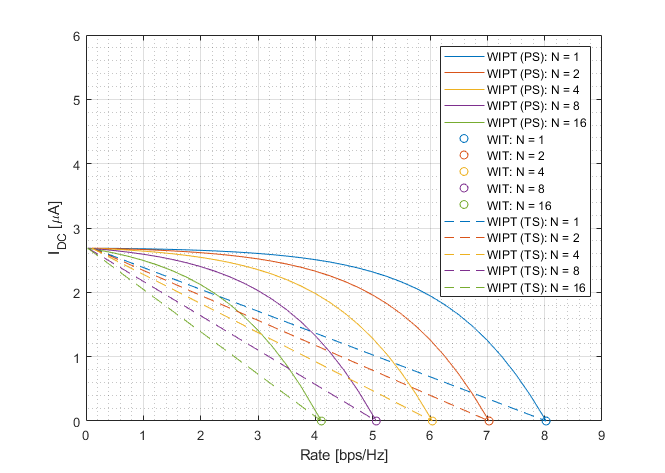
\includegraphics[width=0.48\textwidth]{siso_re_ff_subband_no_power_waveform}}
  \subfigure[FF: No power waveform]{
    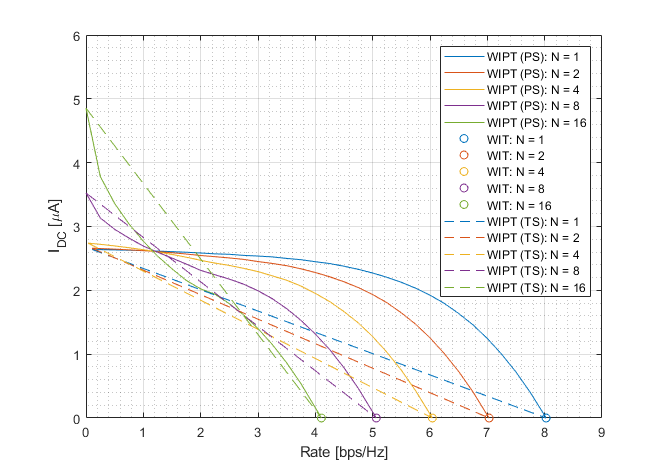
\includegraphics[width=0.48\textwidth]{siso_re_ff_subband_superposed_waveform}}
  \quad
  \subfigure[FS: Superposed waveform]{
    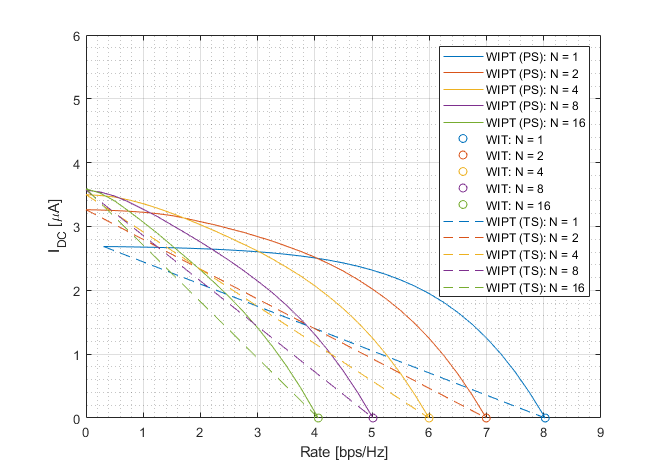
\includegraphics[width=0.48\textwidth]{siso_re_fs_subband_no_power_waveform}}
  \subfigure[FS: No power waveform]{
    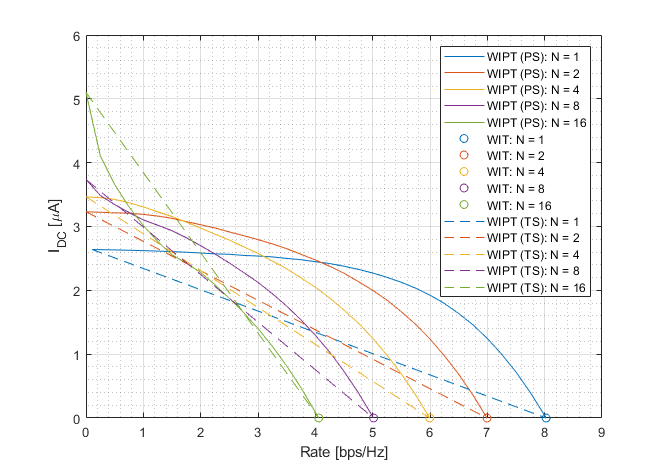
\includegraphics[width=0.48\textwidth]{siso_re_fs_subband_superposed_waveform}}
  \caption{R-E region vs $N$ for FF and FS channels}\label{fig:siso-subband}
\end{figure}

